\documentclass[14pt,a1paper,landscape, margin=8mm, innermargin=5mm,
blockverticalspace=4mm, colspace=5mm, subcolspace=8mm]{tikzposter}\usepackage[]{graphicx}\usepackage[]{color}
%% maxwidth is the original width if it is less than linewidth
%% otherwise use linewidth (to make sure the graphics do not exceed the margin)
\makeatletter
\def\maxwidth{ %
  \ifdim\Gin@nat@width>\linewidth
    \linewidth
  \else
    \Gin@nat@width
  \fi
}
\makeatother

\definecolor{fgcolor}{rgb}{0.345, 0.345, 0.345}
\newcommand{\hlnum}[1]{\textcolor[rgb]{0.686,0.059,0.569}{#1}}%
\newcommand{\hlstr}[1]{\textcolor[rgb]{0.192,0.494,0.8}{#1}}%
\newcommand{\hlcom}[1]{\textcolor[rgb]{0.678,0.584,0.686}{\textit{#1}}}%
\newcommand{\hlopt}[1]{\textcolor[rgb]{0,0,0}{#1}}%
\newcommand{\hlstd}[1]{\textcolor[rgb]{0.345,0.345,0.345}{#1}}%
\newcommand{\hlkwa}[1]{\textcolor[rgb]{0.161,0.373,0.58}{\textbf{#1}}}%
\newcommand{\hlkwb}[1]{\textcolor[rgb]{0.69,0.353,0.396}{#1}}%
\newcommand{\hlkwc}[1]{\textcolor[rgb]{0.333,0.667,0.333}{#1}}%
\newcommand{\hlkwd}[1]{\textcolor[rgb]{0.737,0.353,0.396}{\textbf{#1}}}%
\let\hlipl\hlkwb

\usepackage{framed}
\makeatletter
\newenvironment{kframe}{%
 \def\at@end@of@kframe{}%
 \ifinner\ifhmode%
  \def\at@end@of@kframe{\end{minipage}}%
  \begin{minipage}{\columnwidth}%
 \fi\fi%
 \def\FrameCommand##1{\hskip\@totalleftmargin \hskip-\fboxsep
 \colorbox{shadecolor}{##1}\hskip-\fboxsep
     % There is no \\@totalrightmargin, so:
     \hskip-\linewidth \hskip-\@totalleftmargin \hskip\columnwidth}%
 \MakeFramed {\advance\hsize-\width
   \@totalleftmargin\z@ \linewidth\hsize
   \@setminipage}}%
 {\par\unskip\endMakeFramed%
 \at@end@of@kframe}
\makeatother

\definecolor{shadecolor}{rgb}{.97, .97, .97}
\definecolor{messagecolor}{rgb}{0, 0, 0}
\definecolor{warningcolor}{rgb}{1, 0, 1}
\definecolor{errorcolor}{rgb}{1, 0, 0}
\newenvironment{knitrout}{}{} % an empty environment to be redefined in TeX

\usepackage{alltt}

%----------------------------------------------------------------------------------------
% TIKZPOSTER AND FONT OPTIONS + FIGURE ENVIRONMENT
%----------------------------------------------------------------------------------------

\usetheme{Desert}
\usecolorstyle[colorPalette= BlueGrayOrange]{Spain}
\usetitlestyle{Filled}

%\usebackgroundstyle{Default} %defines the background of the whole poster

%Getting rid of the grading of the title box
\defineblockstyle{Slide}{
    titlewidthscale=1, bodywidthscale=1, titleleft,
    titleoffsetx=0pt, titleoffsety=0pt, bodyoffsetx=0pt, bodyoffsety=0pt,
    bodyverticalshift=0pt, roundedcorners=0, linewidth=0pt, titleinnersep=1cm,
    bodyinnersep=1cm
}{
    \ifBlockHasTitle%
        % changed "right color=..,left color=.." to "fill=blocktitlebgcolor"
        \draw[draw=none, fill=blocktitlebgcolor] 
           (blocktitle.south west) rectangle (blocktitle.north east);
    \fi%
    \draw[draw=none, fill=blockbodybgcolor] %
        (blockbody.north west) [rounded corners=30] -- (blockbody.south west) --
        (blockbody.south east) [rounded corners=0]-- (blockbody.north east) -- cycle;
}

\usepackage{fontspec}
\setmainfont{FreeSerif}
\setsansfont{FreeSans}

\newenvironment{Figure}
    {\par\medskip\noindent\minipage{\linewidth}}
    {\endminipage\par\medskip}

%----------------------------------------------------------------------------------------
% SET KNIT OPTIONS
%----------------------------------------------------------------------------------------



%----------------------------------------------------------------------------------------
% HEADER INFORMATION AND FORMATTING
%----------------------------------------------------------------------------------------

\title{\textbf{\textsc{Cocos Islands}  - \hspace{8pt}Ocean Health Index Project Region Summary Card}}
\institute{National Center for Ecological Analysis and Synthesis}
\author{Generated: Sep 07 2018}
\titlegraphic{
\includegraphics[width=0.7\linewidth]{uploaded_figs/ohi_logo_gradient.png}}

\makeatletter
\renewcommand\TP@maketitle{%
   \begin{minipage}{0.01\linewidth}
   \hfill
   \end{minipage}%
   \begin{minipage}{0.5\linewidth}
        \color{titlefgcolor}
        {\bfseries \LARGE \sc \@title \par}
        {\Large \@institute \par}
    \end{minipage}%
   \hfill
    \begin{minipage}{0.09\linewidth}
    	\centering
           \@titlegraphic
    \end{minipage}
}
\makeatother

\tikzposterlatexaffectionproofoff

%----------------------------------------------------------------------------------------
% DEFINE COLORS
%----------------------------------------------------------------------------------------

\definecolor{mybluegreen}{RGB}{122, 205, 223}
\definecolor{mygreyblue}{RGB}{219, 48, 122}
\definecolor{mylightblue}{RGB}{165, 188, 210}
\definecolor{mydarkgray}{RGB}{64, 79, 88}

%----------------------------------------------------------------------------------------
% START DOCUMENT
%----------------------------------------------------------------------------------------
\IfFileExists{upquote.sty}{\usepackage{upquote}}{}
\begin{document}
\maketitle

%----------------------------------------------------------------------------------------
% FIRST ROW
%----------------------------------------------------------------------------------------

\begin{columns}

\column{0.33}
%\colorlet{blockbodybgcolor}{green!60} %changes color of the complote block
%\colorlet{blocktitlebgcolor}{blue!40} %changes color of the "title" box
%\useblockstyle{Basic} %set blocks to a basic style (round corners, solid title...)

\block{\textbf{\textsc{What is the Ocean Health Index (OHI)?}}
\item[]{The OHI is a scientific framework used to measure how healthy oceans are. Understanding the state of our oceans is a first step towards ensuring they can continue providing humans benefits now and in the future.}}
{%

\begin{tikzfigure}[Caption with explanation of what it is.]
\includegraphics[width=0.8\linewidth]{example-image}
\end{tikzfigure}
}

\column{0.34}
\block{\textbf{\textsc{Why is it important?}}
\item[] {The ocean plays a critical role in supporting human well-being from providing food to regulating global climate. This index provides a powerful tool to raise public awareness, direct resource management, improve policy and prioritize scientific research. 
}}
{%
\begin{tikzfigure}[Caption with explanation of what it is.]
\includegraphics[width=0.8\linewidth]{example-image}
\end{tikzfigure}
}



%----------------------------------------------------------------------------------------
% SECOND ROW
%----------------------------------------------------------------------------------------

\begin{columns}
\column{0.5}
\block{\textbf{\textsc{OHI Goals}}
\item[] {Ocean health is defined as the sustainable delivery of ten widely-held public goals for ocean ecosystems}}
{
\begin{itemize}
\item[] \textbf{\textsc{Artisanal Opportunity (AO)}} Opportunity for small-scale fishers to supply catch to local communities or sell in local market.
\item[] \textbf{\textsc{Biodiversity (BD)}} Conservation status of marine species and key habitats, which inform about the rest of species that depend on them.
\item[] \textbf{\textsc{Carbon Storage (CS)}} Condition of coastal habitats that store and sequester atmospheric carbon.
\item[] \textbf{\textsc{Clean Water (CW)}} Degree to which oceans are free of chemicals contaminants, excessive nutrients, human pathogens and trash.
\item[] \textbf{\textsc{Livelihoods and Economies (LE)}} Coastal and ocean-dependent livelihoods (job quantity and quality) and economies (revenues) produced by marine sectors.
\item[] \textbf{\textsc{Coastal Protection (CP)}} The amount of protection provided by marine and coastal habitats serving as natural buffers against incoming.
\item[] \textbf{\textsc{Food Provision (FP)}} The sustainable harvest of seafood from wild-caught fisheries and mariculture.
\item[] \textbf{\textsc{Natural Products (NP)}} The natural resources that are sustainably extracted from living marine resources.
\item[] \textbf{\textsc{Sense of Place (SP)}} The conservation status of iconic species and geographic locations that contribute to cultural identity.
\item[] \textbf{\textsc{Tourism and Recreation (TR)}} The value people have for experiencing and enjoying coastal areas and attractions.
\end{itemize}
}

\column{0.5}

\block{\textbf{\textsc{Regional Goal Scores Over Time}} 
\item[]{Every year, previous scores are re-calculated with the most recent methods.}}
{%
\begin{Figure}[Scores over time using the 2018 methods.]
\begin{knitrout}
\definecolor{shadecolor}{rgb}{0.969, 0.969, 0.969}\color{fgcolor}\begin{kframe}


{\ttfamily\noindent\color{warningcolor}{\#\# Warning: Removed 7 rows containing missing values (geom\_path).}}

{\ttfamily\noindent\color{warningcolor}{\#\# Warning: Removed 7 rows containing missing values (geom\_point).}}\end{kframe}
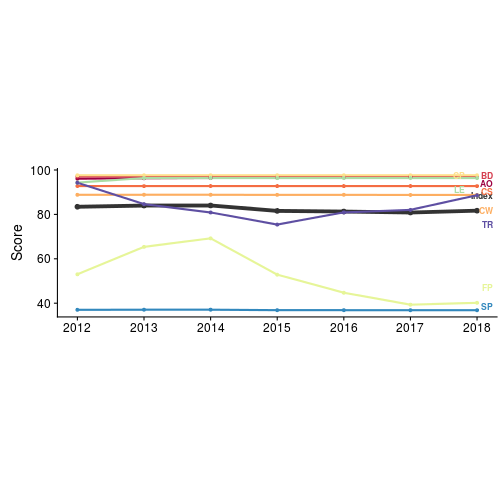
\includegraphics[width=\maxwidth]{figure/rgn_ts_plot-1} 

\end{knitrout}
\end{Figure}
}

\end{columns}

%----------------------------------------------------------------------------------------
% END DOCUMENT
%----------------------------------------------------------------------------------------

\end{document}
